\documentclass{classrep}
\usepackage[utf8]{inputenc}
\frenchspacing

\usepackage{graphicx}
\usepackage[usenames,dvipsnames]{color}
\usepackage[hidelinks]{hyperref}
\usepackage{lmodern}
\usepackage{graphicx}
\usepackage{placeins}
\usepackage{url}
\usepackage{amsmath, amssymb, mathtools}
\usepackage{listings}
\usepackage{fancyhdr, lastpage}

\pagestyle{fancyplain}
\fancyhf{}
\renewcommand{\headrulewidth}{0pt}
\cfoot{\thepage\ / \pageref*{LastPage}}

%--------------------------------------------------------------------------------------%
\studycycle{Informatyka stosowana, studia dzienne, II st.}
\coursesemester{I}

\coursename{Wprowadzenie do Data Science i metod uczenia maszynowego}
\courseyear{2020/2021}

\courseteacher{mgr inż. Rafał Woźniak}
\coursegroup{Wtorek, 13:15}

\author{%
    \studentinfo[239661@edu.p.lodz.pl]{Szymon Gruda}{239661}
}

\title{Zadanie 1.: Problem Set 1}

\begin{document}
    \maketitle
    \thispagestyle{fancyplain}

    \section{Wprowadzenie} {
        Dane wraz ze wykorzystującą je statystyką pozwalają opisywać otaczający ludzi świat i informować co się w nim dzieje.
         Bardzo ważnym aspektem jest ich prezentacja (wizualizacja). Dużo trudniej jest ludziom zinterpretować długą tabelę 
         z samymi liczbami, lepszą metodą jest zwizualizowanie danych, np. poprzez wykres. Niestety wizualizowanie danych jest 
         podatne na różnego rodzaju manipulacje, które zostaną omówione poniżej.
    }

    \section{Przykłady manipulacji danymi podczas ich wizualizacji} {
        \begin{figure}[!htbp]
            \centering
            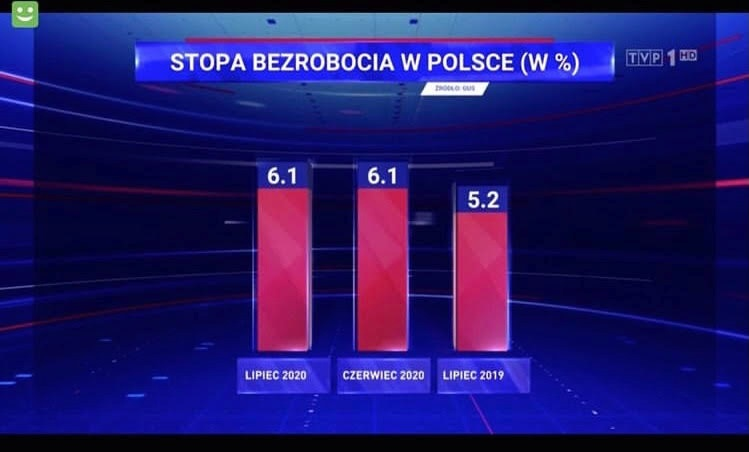
\includegraphics
            [width=0.9\textwidth,keepaspectratio]
            {img/1.jpg}
            \caption
            {Wykres stopy bezrobocia w Polsce}
            \label{rysunek1}
        \end{figure}
        \FloatBarrier
       Rysunek \ref{rysunek1} przedstawia wykres stopy bezrobocia w Polsce.
       Wykres na pierwszy rzut oka wskazuje, że stopa bezrobocia maleje. Niestety tak nie jest, okazuje się że autor wykresu,
        miesiąc chronologicznie późniejszy umieścił wcześniej. Dodatkowo dziedzina danych to bardzo wąski zbiór trzech miesięcy,
        przez co wykres nie obrazuje sytuacji w ciągu całego jednego roku, dopuszczalne byłoby przedstawienie danych zebranych
        w ramach jednego kwartału, ale nie trzech różnych miesięcy, na przestrzeni dwóch lat.
       
        \begin{figure}[!htbp]
            \centering
            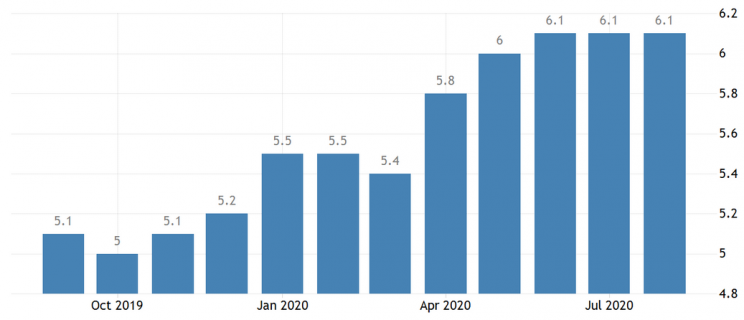
\includegraphics
            [width=0.9\textwidth,keepaspectratio]
            {img/1fixed.png}
            \caption
            {Wykres stopy bezrobocia w Polsce zaprezentowany w sposób poprawny}
            \label{rysunek1fixed}
        \end{figure}
        \FloatBarrier
       Rysunek \ref{rysunek1fixed} również przedstawia wykres stopy bezrobocie w Polsce, jest on natomiast pozbawiony wad wykresu
        z rysunku \ref{rysunek1}.
       
        \begin{figure}[!htbp]
            \centering
            
\includegraphics
            [width=0.9\textwidth,keepaspectratio]
            {img/2.jpg}
            \caption
            {Wykres liczby stop cafe w Polsce}
            \label{rysunek2}
        \end{figure}
        \FloatBarrier
       Rysunek \ref{rysunek2} przedstawia "dynamniczny wzrost liczby stop cafe w Polsce".
        Infografika nie zawiera dokładnej informacji co prezentuje, ale można się domyślać że liczbę kawiarni na przestrzeni dwóch lat.
        Liczby zostały przedstawione jako dwa kubki kawki, jeden jest czterokrotnie mniejszy od drugiego.
        Czytelnik mógłby wywnioskować na podstawie samej grafiki, że ma doczynienia z dwukrotnym wzrostem liczby, otóż nie,
        podane obok kubków liczby prezentują wzrost liczby kawiarni o 2.
       \begin{figure}[!htbp]
            \centering
            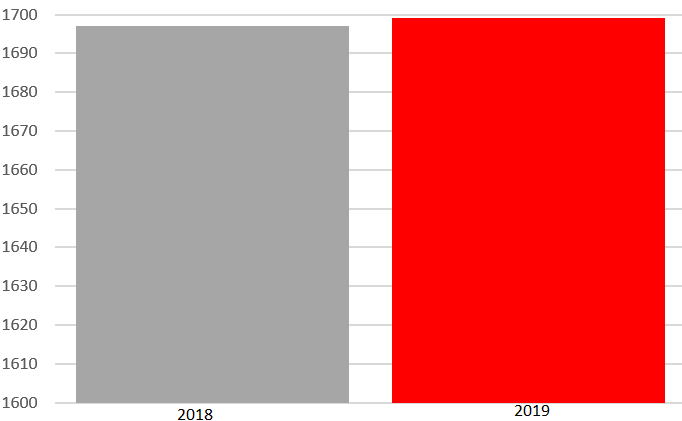
\includegraphics
            [width=0.9\textwidth,keepaspectratio]
            {img/2fixed.png}
            \caption
            {Poprawiony wykres liczby stop cafe w Polsce}
            \label{rysunek2fixed}
        \end{figure}
        \FloatBarrier
        Rysunek \ref{rysunek2fixed} przedstwia wykres liczby kawiarni na przestrzeni dwóch lat, 
        pozboawiony wad wykresu z rysunku \ref{rysunek2}.
}

    
    \section{Wnioski} {
        Wykonując zadanie można wywnioskować, że:
        \begin{itemize}
            \item Nieodpowiednią wizualizacją danych można przedstawić dowolną informację, wykorzystując niepasujące do niej dane.
            \item Bardzo istotnym czynnikiem w wizualizcji danych jest okres czasu, z którego dane będą prezentowane.
            \item Szczególną uwagę należy zwracać na informacje uzyskiwane z infografik, ponieważ zbyt skupiony na ładnym przedstawianiu danych autor, może zrobić to w sposób nierzetelny.
        \end{itemize}
    }

\end{document}
